\chapter{基于 Android 平台的心电监护系统的设计与实现}
\section{系统功能需求分析 }
基于 Android 平台的心电监护系统的主要功能是以文字与曲线的形式为用户提供心电信号的状态检测服务,并在此基础上以友好的方式与用户进行人机交互,
让用户及时了解心电信号的特征信息\cite{23,24,25,26}。根据需求分析其功能主要包括: 

(1)	预读数据。将需处理的数据提前与程序打包,程序在工作的时候直接调用数据。 

(2)	数据滤波。对读入的原始数据进行预处理,包括滤波去噪、去除基线漂移干扰等。 

(3)	特征提取。对预处理后的数据按照心电特征值相关提取算法,计算并保存相应的结果。 

(4)	心电波形绘制与特征点标注。按照一一对应的关系,分别动态绘制出预处理前后的数据波形,并在预处理后数据的图像中动态标记上步检测出的相关特征。 

(5)	心电特征结果显示。将(3)中分析得到的各项心电特征值以直观明了、简单易懂的方式呈现给用户,且给出必要的说明。 

(6)	操作简单。尽量使用常规操作完成应用,方便大众人群使用。 

\section{系统的Java类设计与工作流程示意 }
Eclipse 下的 Android 工程文件如\autoref{fig:501}所示。src 是源文件目录,对应 4 个 Java 类;assets 是静态资源文件目录,存储了需处理的原始数据;
res 是资源文件目录,包含布局文件、图片等内容。 

源文件目录下的 4 个 Java 类分别完成的功能如下: 

(1)	Drawecgwave: Service 类,负责滤波前后心电波形的对比显示,并完成特征点的标记工作。 

(2)	Ecgdetect: Service 类,负责对心电数据(滤波后数据)进行特征提取。 

(3)	MainActivity: Activity 类,程序的整体运行起点。同时负责提取得到的特征显示。 

\begin{figure}[htbp]
    \centering
    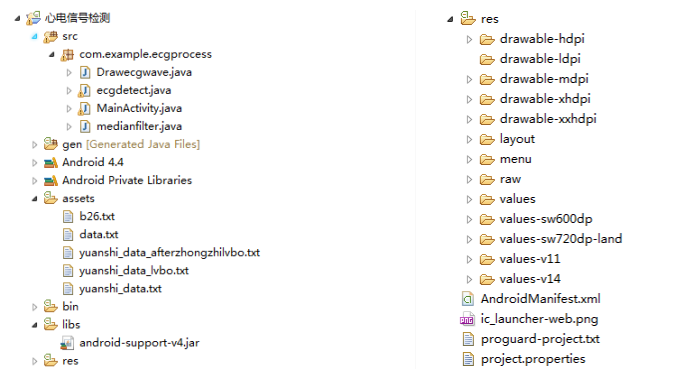
\includegraphics[width=.8\linewidth]{501}
    \caption{\label{fig:501} Android 工程文件}
\end{figure}
\begin{figure}[htbp]
    \centering
    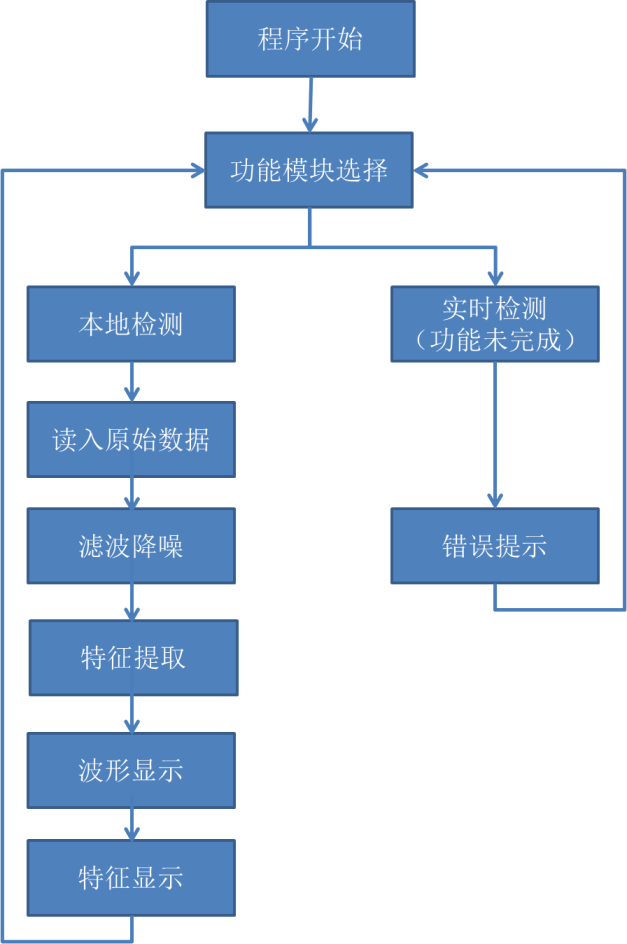
\includegraphics[width=.5\linewidth]{502}
    \caption{\label{fig:502} 系统工作流程图 }
\end{figure}

(4)	Medianfilter: Service 类,负责对心电数据(原始数据)进行滤波降噪处理。 

根据以上的需求分析与功能要求,系统整体运行的流程图如\autoref{fig:502}所示。 

\section{系统布局与UI界面的设计}
根据系统流程图可知,系统输入是用户人工选择的两种工作模式,系统的输出包括心电信号波形输出与心电特征值的数值输出。根据 Android 组件的相关特性,
本文将选择工作模式设计为 Button 部件,心电波形的显示设计为 Surfaceview 部件,特征值的输出设计为 Textview 部件。系统的整体布局文件采用竖直方向的线性布局方式。系统最终
UI 界面效果如\autoref{fig:503}所示。 
\begin{figure}[htbp]
    \centering
    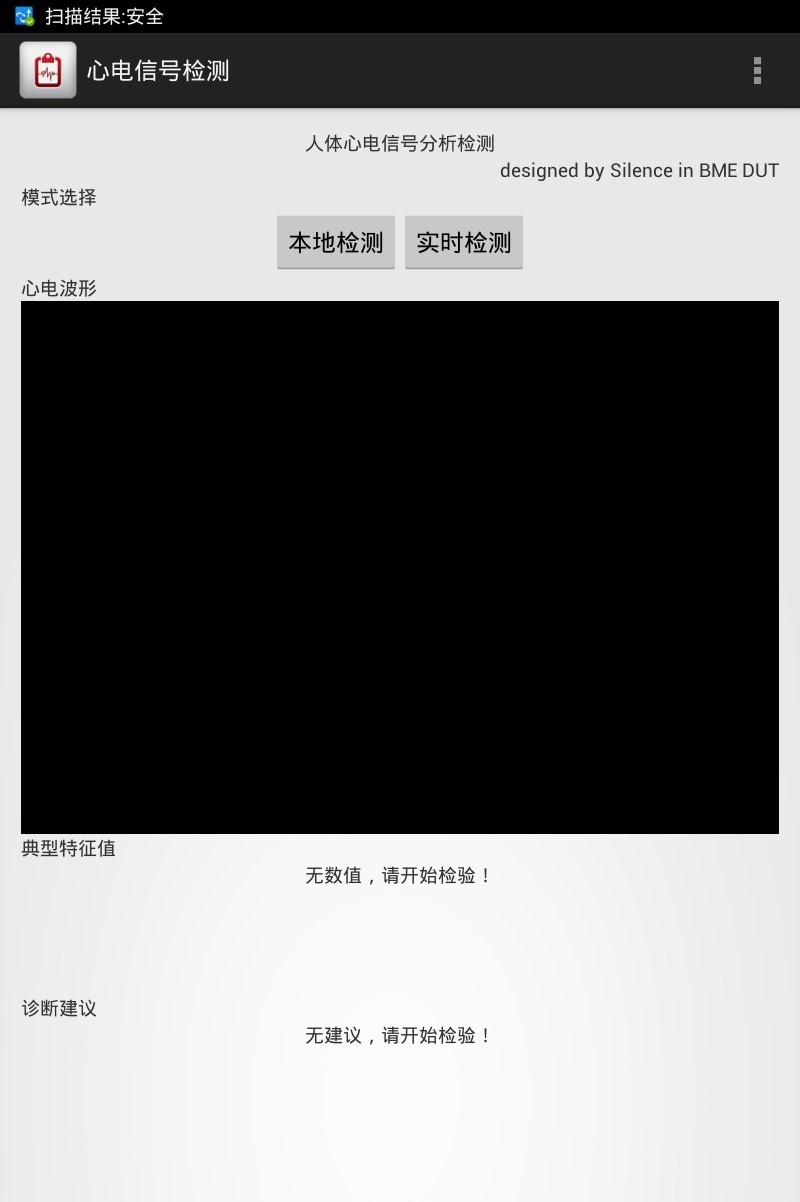
\includegraphics[width=.6\linewidth]{503}
    \caption{\label{fig:503} 心电监测系统 UI 界面}
\end{figure}

\section{绘图的实现及改进优化}
\subsection{Android下绘图的基本知识} 
Android 框架 API(Application Programming Interface,应用程序编程接口)提供一组二维绘画 API,允许开发者渲染自定义图形到一个画布上或者修改现存的 
View 以自定义绘图操作\cite{27}。当绘画二维图形时,Android 提供了以下两种方式: 

(1)	在布局文件里定义的 View 对象上绘画图形或动画。在这种方式下,图形绘画过程由系统的正常 View 层级绘画过程处理完成。开发者仅需定义要在 View 对象上所需的图形即可。 

(2)	直接在一个 Canvas 对象上绘制图形。在这种方式下,开发者需要预先定义合适的图形绘制的$onDraw()$方法(用以控制在 Canvas 的绘图方法)
或 Canvas 的其中一个 $draw...()$方法(如 $drawPicture()$等)。此外,在此方法下,开发者还可以控制绘制动画,实现动态绘图功能。  

由于在绘图过程中需根据数据点绘制所需波形,因此,本系统的设计过程中选取了后一种方法。同时为满足波形动态绘制的需要,我们需要在布局文件中创建一个 SurfaceView 
以进行相应的绘图。SurfaceView 是一个特殊的 View 子类,它提供 View 层级内的一个专用绘画表面。该绘画表面可以供应用程序的第二线程调用绘图,使应用程序不需要等待
系统准备工作就绪就可以绘画。换言之,一个使用了 SurfaceView 的子线程可以按其自身的速度在其 Canvas 上处理完成来绘画。 

画布(Canvas)是图形编程中一个最基本概念,通常由两个基本的绘图组件组成: 

(1)	Canvas  
Canvas 类封装了用作绘图表面的位图,可以向底层的位图绘制基本图形。此外它还提供了 $draw...()$方法来实现设计。\autoref{tab:501}对 Canvas 提供了绘图方法进行了简要说明。 

\begin{longtblr}
    [
        theme          = {dut},
        caption        = {Canvas 的常用绘图方法},
        label          = {tab:501},
    ]
    {
        colspec        = {X[1,c,m]X[1,c,m]},
        hline{1,Z}     = {\thickline},
        hline{2}       = {\thinline},
        rowhead        = 1,
        row{odd}       = {bg=\oddcolor}, 
        row{even}      = {bg=\evencolor},
        row{1}         = {font=\headfont,bg=\headcolor},
        row{2-Z}       = {font=\nonheadfont},
    }
    方法函数 &  功能\\
    drawARGB/drawRGB/drawColor 	&   使用单一的颜色填充画布。 \\
    drawArc 	&   在一个矩形区域的两个角之间绘制一个弧。  \\
    drawBitmap 	&   在画布上绘制一个位图。                   \\
    drawBitmapMesh 	&   使用一个 mesh(网)来绘制一个位图。  \\
    drawCircle 	&   以给定的点为圆心,绘制一个指定半径的圆。  \\
    drawLine(s) 	&   在两个点之间画一条(多条)直线。  \\
    drawOval 	&   以指定的矩形为边界,画一个椭圆。  \\
    drawPaint 	&   使用指定的 Paint 填充整个 Canvas。  \\
    drawPath 	&   绘制指定的 Path。  \\
    drawPicture 	&   在指定的矩形中绘制一个 Picture 对象。  \\
    drawPosText 	&   绘制指定了每一个字符的偏移量的文本字符串。  \\
    drawRect 	&   绘制一个矩形。  \\
    drawRoundRect 	&   绘制一个圆角矩形。  \\
    drawText 	&   在 Canvas 上绘制一个文本串。  \\
    drawTextOnPath 	&   在一个指定的 path 上绘制文本。  \\
    drawVertices 	&   绘制一系列三角形面片,通过一系列顶点来指定它们。  \\
\end{longtblr}

(2)	Paint  

Paint 类相当于一个笔刷和调色板,可以将指定如何将基本图形绘制到位图上。表中的绘图方法都需要指定一个 Paint 对象来渲染它。Paint 可以选择如何使用上面描述的 
draw 方法来渲染绘制在画布上的基本图形。通过修改 Paint 对象,可以在绘图的时候控制颜色、样式、字体和特殊效果。除了这些简单的控制之外,
Paint 类还支持透明度,另外,它也可以通过使用各种各样的阴影、过滤器和效果进行修改,从而提供由更丰富的、复杂的画笔和颜料组成的调色板。
此外,Paint 还提供了对 PathEffect 的支持,可以通过其控制绘制轮廓(线条)的方式。而在绘制斜线或文本时,为了保证所绘制斜线外观上的平滑与
及绘制的文字可读性更强,还可以通过 Paint 提供的抗锯齿效果来实现此需求。 

在布局文件中创建了 SurfaceView 之后,在 SurfaceView 上新建一个 Canvas 后,就可以使用通过定义好 Paint 的对象在 Canvas 上调用 
Canvas 的各种方法进行绘图。如图\autoref{fig:504}所示,由于 Android 绘图的机制是按像素点进行,而像素点分别按照水平方向与竖直方向取正整数值,
且通常 Canvas 的左上角是坐标原点。如果直接进行绘制,绘制出的图像是沿 Canvas Y 轴向下的,不符合人们通常的视觉习惯。
而在本文设计所需绘制的数据点一般幅值不超过 3。而 Surfaceview 在真机上的大小一般是 100 数量级的,为充分利用 Surfaceview 空间,
同时解决上述图像倒置与图像不够清楚的问题,在本文的实际绘图之前,需要对所需绘制的数据进行一次映射,映射关系如所示。 
\begin{equation}
    \label{equ:501}
    x[i]= i \mathop{mod} width
\end{equation}
\begin{equation}
    \label{equ:502}
    y[i]= k * data[i] + b
\end{equation}

其中 $data$ 为所需绘制的数据点所存的数据,$i$ 为其下标,$x[i]$与 $y[i]$是其对应 Surfaceview 上的横纵坐标值,$k$ 为调幅因子,作用是调整图像方向及实现放大图像,其值为负,具 
体值的大小需要视与 Surfaceview 的高度与数据点幅值关系确定,$b$ 为位移因子,作用是使图像居中显示,其值为正,与 Surfaceview 的高度处于同一数量级。 
\begin{figure}[htbp]
    \centering
    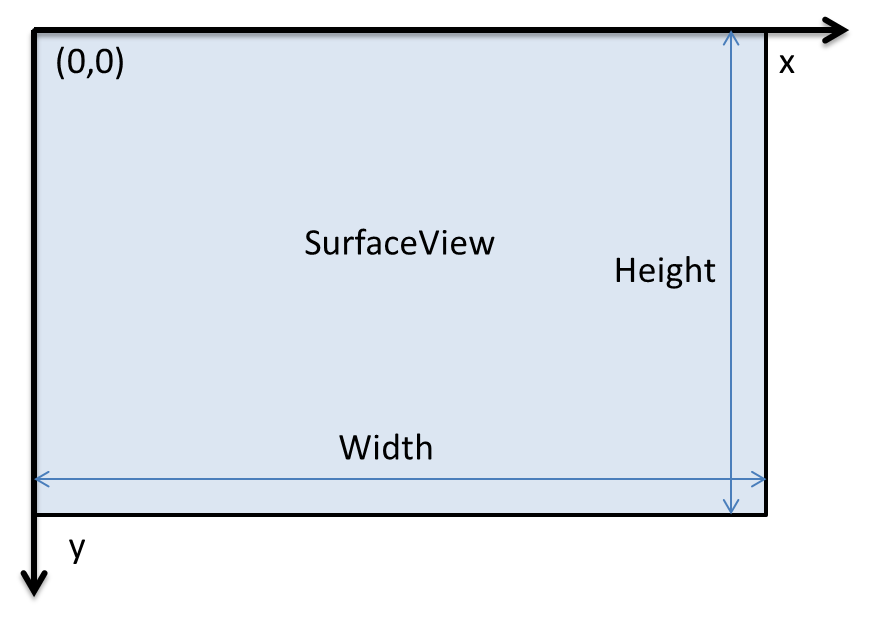
\includegraphics[width=.8\linewidth]{504}
    \caption{\label{fig:504}Surfaceview 示意}
\end{figure}

\subsection{绘图过程中技术问题及解决方案} 

(1)	单点绘图与一次性绘制图形 

在数据的绘图过程中,本文最开始的思路是外层嵌套循环,每次取出数据的两个点,使用 Canvas 的 $drawline()$函数进行绘制。事实证明这样的思路的确是可行的,
在智能手机上的执行效果如图\autoref{fig:5051}所示,但绘制的波形效率低下,绘制完 3000 个点的数据时间将近 10s。分析造成这种情况的原因主要体现在两个方面,
首先数据是按每两点取出的并绘制从而导致外层的循环次数过多。其次,绘图时反复锁定提交 Canvas、绘制、提交 Canvas 造成了大量的时间浪费。 
\begin{figure}[htbp]
    \centering
    \subfigure[\label{fig:5051}$drawline()$函数绘图效果]{
    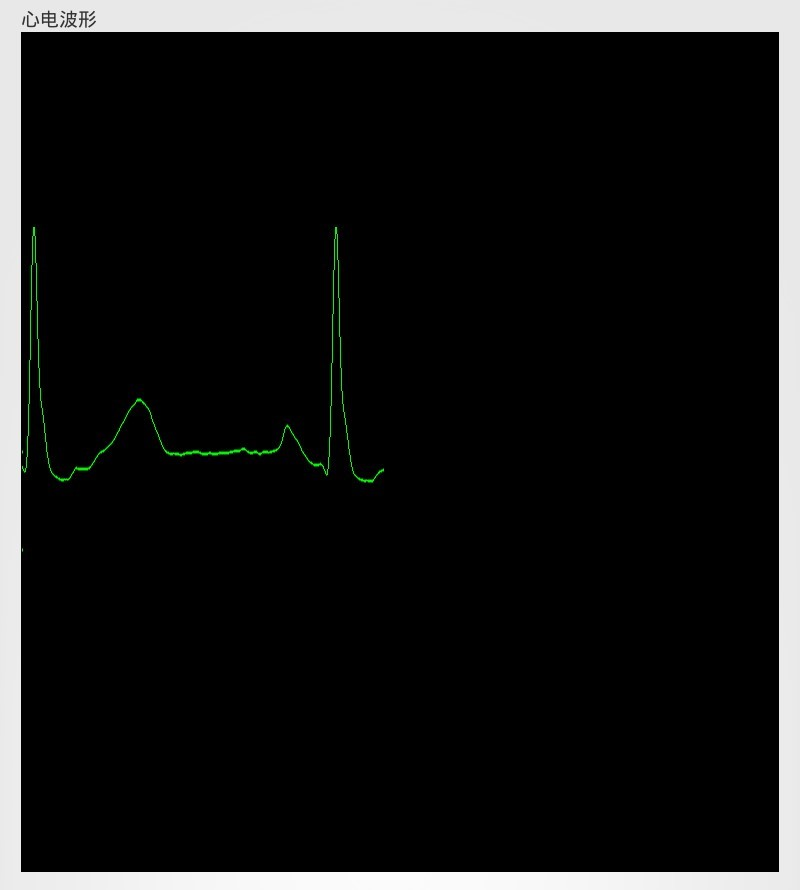
\includegraphics[width=7cm]{5051}
    }
    \quad
    \subfigure[\label{fig:5052}$drawlines()$函数绘图效果]{
    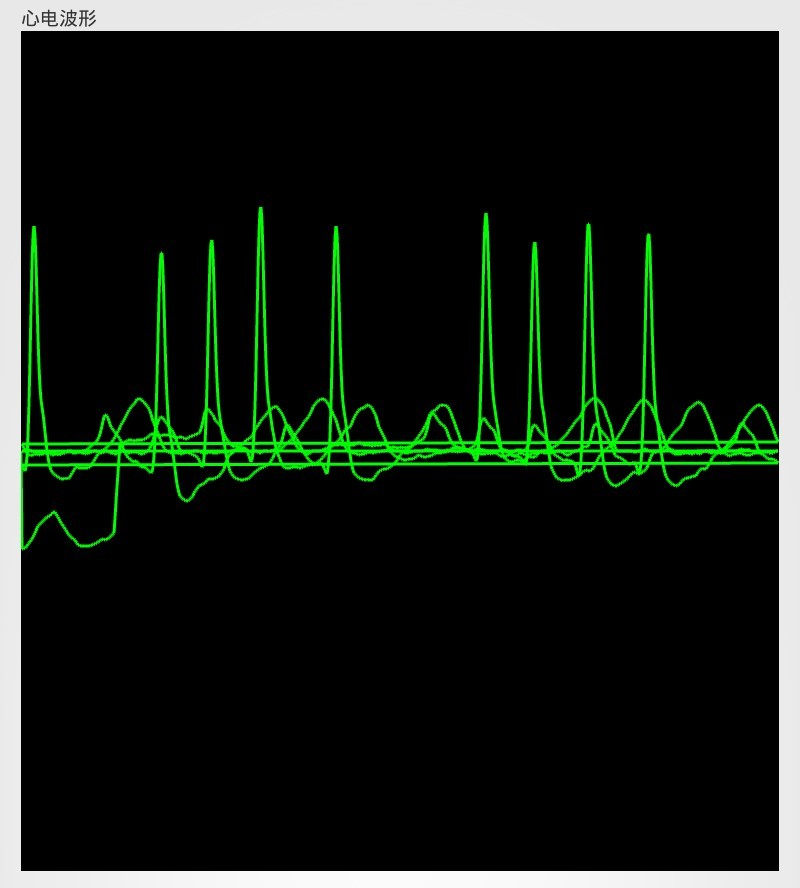
\includegraphics[width=7cm]{5052}
    }
    \caption{\label{fig:505}单点绘图与多点绘图效果对比}
\end{figure}

解决优化方案是考察了 Canvas 提供的 $drawlines()$函数,在调用之前直接将所需绘制的直线的起始点坐标依次保存在一维数组里,绘制时只需一次锁定 Canvas、
一次性绘制完所有直线、一次性提交 Canvas 并显示。如图\autoref{fig:5052}所示,优化后的方法极大的提高了时间效率, 对 3000 点的绘制基本上实现了ms级别的绘图速度。
作为效率对比,图中暂时没有考虑清屏及首尾点之间横线的处理问题。

(2)	波形的单屏满显示与动态显示 

如图\autoref{fig:5052}所示,调用 $drawlines()$函数一次性计算所有需绘制的直线时,会出现单屏重复显示及多余的的首尾点之间横线。解决方法是,每次绘制图形时,
仅按当面屏幕的横向像素值从原始数据中取数计算出相应的直线将其坐标保存在 $drawlines()$函数的入口参数数组中,处理好当前屏幕的所需绘制的斜线。如图\autoref{fig:5061}
所示,这样就可以完美解决单屏满显示。 
\begin{figure}[htbp]
    \centering
    \subfigure[\label{fig:5061}单屏显示的波形]{
    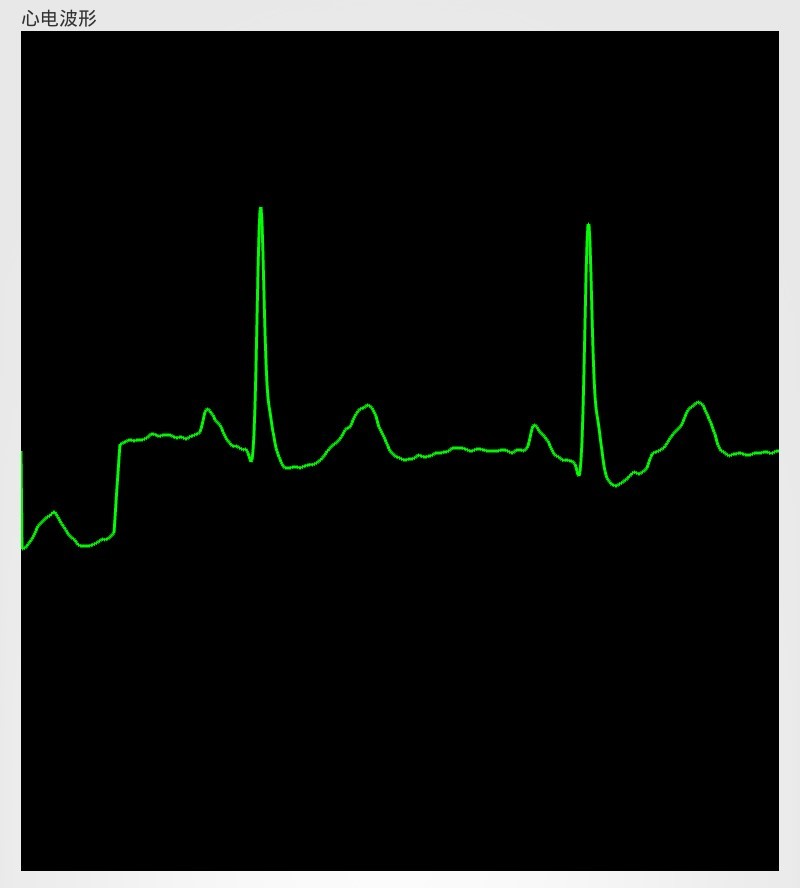
\includegraphics[width=7cm]{5061}
    }
    \quad
    \subfigure[\label{fig:5062}左图波形数据左移若干数值后的波形图]{
    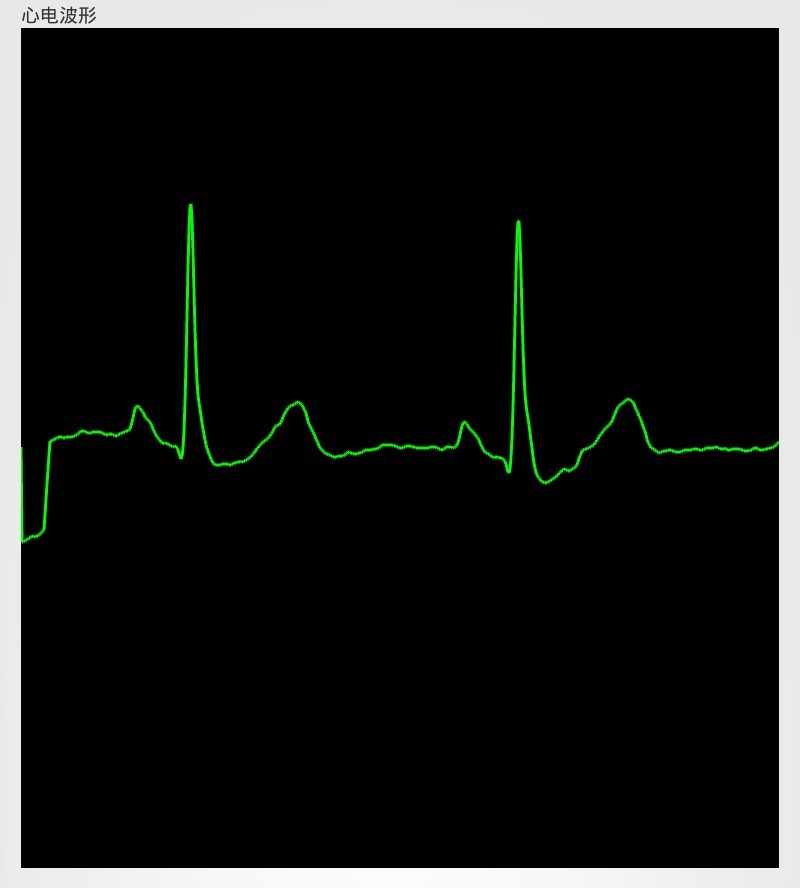
\includegraphics[width=7cm]{5062}
    }
    \caption{\label{fig:506}单屏满显示与动态绘图的实现}
\end{figure}

为了能让绘制的图像“运动”起来,这里我们运用了人体视觉的暂留效应。暂留效应,也称视觉惰性,是指光象一旦在视网膜上形成,视觉将会对这个光象的感觉维持一个有限的时间,
对于中等亮度的光刺激,视觉暂留时间约为 0.05 至 0.2 秒。因此在图像的绘制过程中,如果我们对每次绘制的一屏的数据的起始点做一定步进,但保证绝大多数点依然与
上一屏绘制的数据点相同,只是在屏幕上的位置关系发生变化。这样在视觉暂留效应下,整体的图像就会看起来从右向左开始“运动”起来,如\autoref{fig:506}所示。 

(3)	网格与坐标轴 

为使波形图像有更直观的显示,我们给显示的曲线增加了网格线及坐标轴。实现的具体方法是,在绘制完图像点之后并不直接提交图像,而是每次固定的进行
绘制坐标轴及网格线后再进行图像的提交。也就是说,在整个绘图过程中,坐标轴与网格线是不停地在固定位置反复绘制的。最后实现的效果如\autoref{fig:507}所示。 
\begin{figure}[htbp]
    \centering
    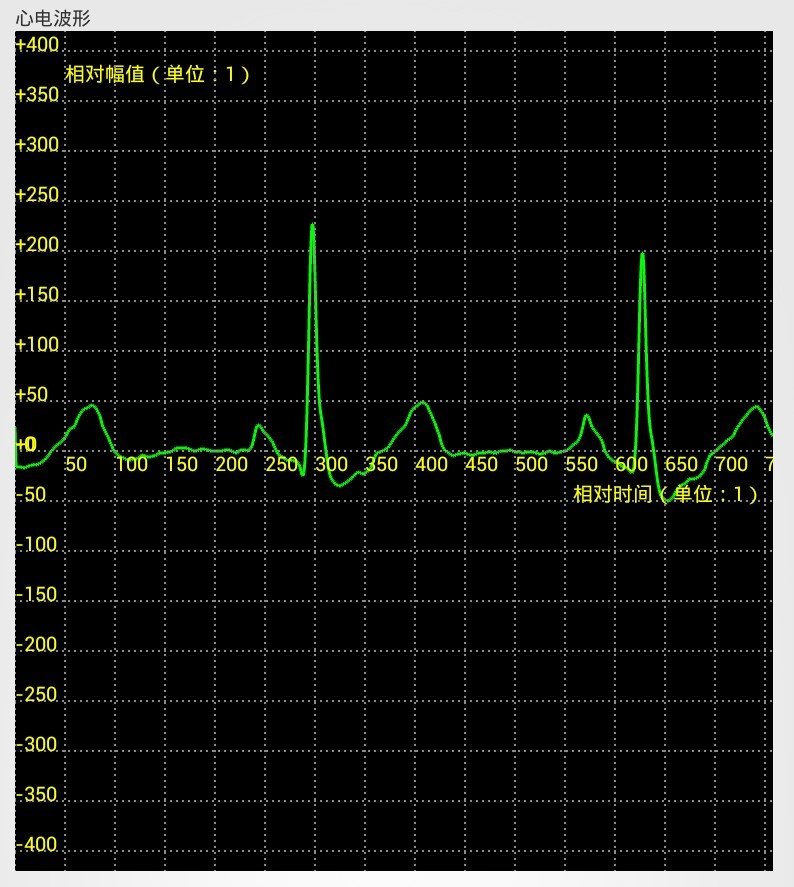
\includegraphics[width=.7\linewidth]{507}
    \caption{\label{fig:507}网格线与坐标轴实现 }
\end{figure}
\begin{figure}[htbp]
    \centering
    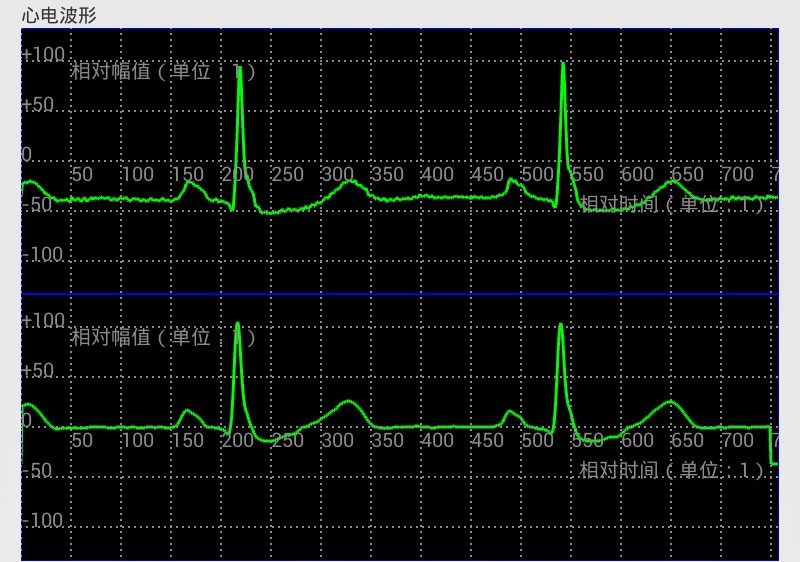
\includegraphics[width=.7\linewidth]{508}
    \caption{\label{fig:508}双屏显示的实现}
\end{figure}

(4)	双屏显示 

在程序最开始的设计中,我们是按先显示原始数据再显示滤波后数据的顺序进行的,但这样无法直观了观测到滤波的实际效果。为了有更直观的对比,
我们需要将两者按照相同的时间步进进行显示。具体实现的过程中考察了多种方法的效果,包括创建两个 Surfaceview 同时引入线程的概念,
不停的在两个线程间切换,交替绘图,但实际运行时效果较差出现了闪屏现象。最终采用的方法是调整 5.1 小节中提及的映射关系式,使滤波前后的
两组数据分别映射在屏幕的上下部,并各自以上下部的中心为水平轴绘图。此方法能很好的解决闪屏现象,\autoref{fig:508}展示了最终实际的效果。 

(5)	特征标注 

为对程序中涉及的心电特征检测程序的准确率进行直观的评价,我们需要在图中进行相应的标注工作。由于相关检测算法已将相关特征值在滤波后
的数组中下标值记录,在绘制图形当前一屏的数据时,对数据点进行一遍遍历,比照绘制的点下标与特征值是否相同,如果相同,则在该点处绘制
标记特定的符号,并按照波形动态显示的类似方法实现随图像动态“运动”。 

但在实现时最开始会出现所有特征点均能显示一次,无法随波形运动,如\autoref{fig:509}所示。检查程序发现,这是由于遍历当前屏幕点的时候对特征点的遍历
只进行了一次,修改成遍历当前屏幕点时每次均从头遍历相关特征值数组,即可实现特征点的动态标注,如\autoref{fig:510}所示。 
\begin{figure}[htbp]
    \centering
    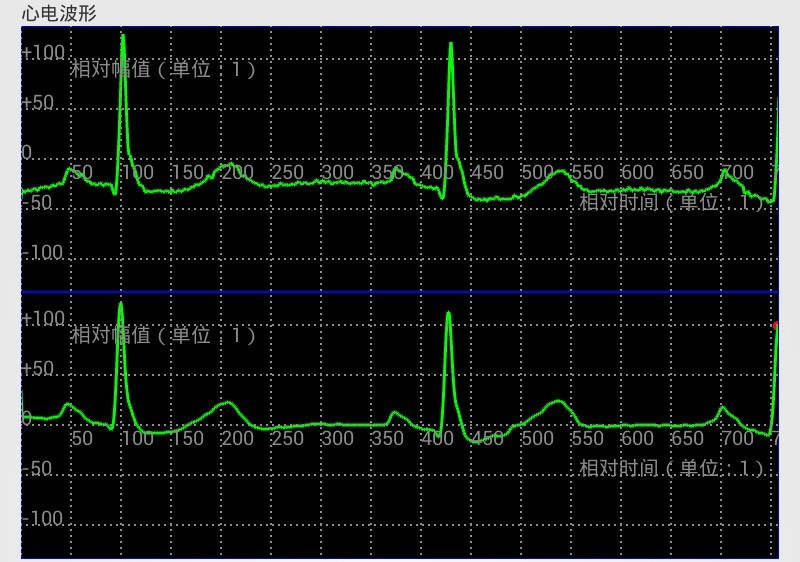
\includegraphics[width=.7\linewidth]{509}
    \caption{\label{fig:509}特征标注时仅在第一次标注(在下方波形的R峰第一次出现时有标记点)}
\end{figure}

\begin{figure}[htbp]
    \centering
    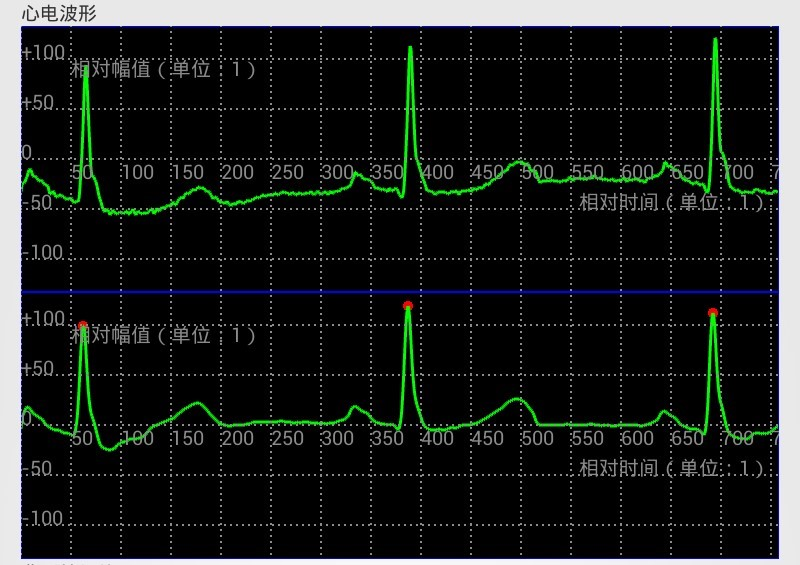
\includegraphics[width=.7\linewidth]{510}
    \caption{\label{fig:510}动态标注特征的实现(在下方波形的每个R峰均有标记点)}
\end{figure}

\begin{figure}[htbp]
    \centering
    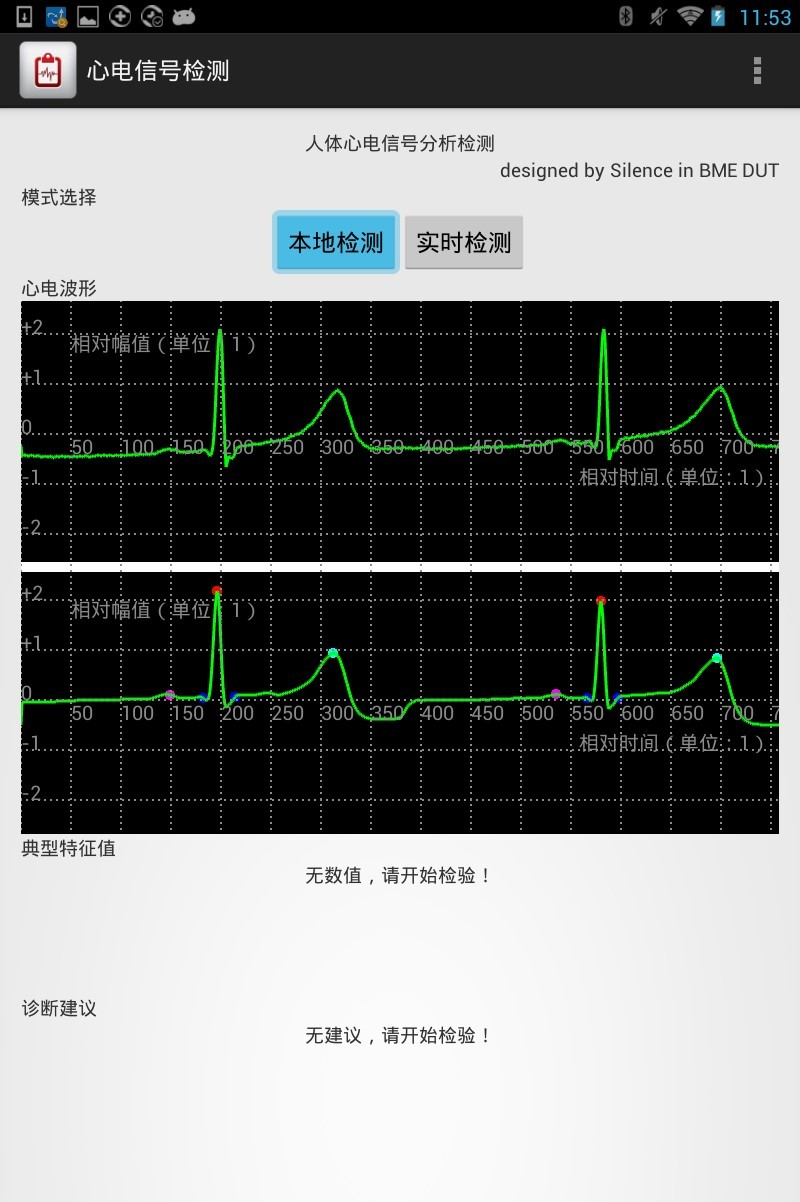
\includegraphics[width=.55\linewidth]{511}
    \caption{\label{fig:511}系统运行数据显示的效果}
\end{figure}
\section{系统运行效果}
运行程序后,点击本地检测按钮,即可开始数据分析功能,系统将对原始数据滤波前后的波形进行对比显示,
同时在滤波后的波形图中动态标注检测出的特征值。在显示完所有数据后将对相关特征值及计算得到心律数据进行文本显示,
整个过程如\autoref{fig:511}、\autoref{fig:512}所示。 

\begin{figure}[htbp]
    \centering
    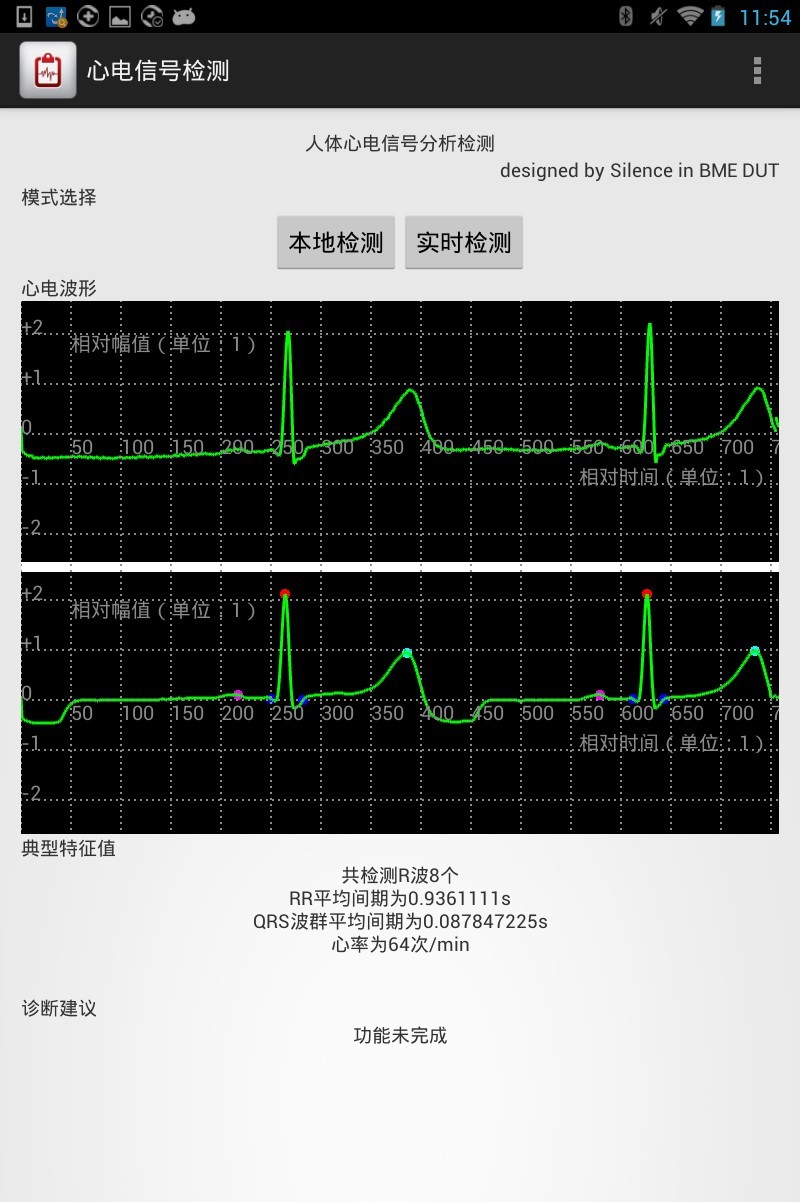
\includegraphics[width=.55\linewidth]{512}
    \caption{\label{fig:512}系统运行后结果显示效果 }
\end{figure}

\section{本章小结}
本章介绍了基于智能手机的心电监护系统的具体实现过程,首先从设计要求、预期的功能开始,对系统做出了简单的概要。随后从具体的开发过程入手,从界面设计、系统流程等环节,详细介绍了系统的整体设计思路并绘图功能一项的具体实现及改进优化过程为例,有代表性的介绍了软件开发过程中具体实现时遇到的技术问题及解决方案。
最后给出了系统运行的效果示意。 
